\documentclass[10pt]{article}
\usepackage[margin=0.75in]{geometry}
\usepackage[T1]{fontenc}
\usepackage{lmodern}
\usepackage{amsmath,amssymb,amsthm,mathtools}
\usepackage{booktabs,longtable,array}
\usepackage{graphicx}
\usepackage{xcolor}
\usepackage{enumitem}
\usepackage{algorithm}
\usepackage{algpseudocode}
\usepackage[hidelinks]{hyperref}
\usepackage{url}
\usepackage{cleveref}
\graphicspath{{figures/}{../engine/figures/}}
\def\UrlBreaks{\do\/\do-\do\_\do.}
\setlist{nosep,leftmargin=*}
\setlength{\parskip}{2pt}
\renewcommand{\arraystretch}{1.08}
\renewcommand{\topfraction}{0.92}\renewcommand{\bottomfraction}{0.8}\renewcommand{\textfraction}{0.06}
\renewcommand{\floatpagefraction}{0.85}\setcounter{topnumber}{3}\setcounter{totalnumber}{5}

% ---------------------------------------------------------------- theorem environments (shared counter)
\theoremstyle{plain}
\newtheorem{theorem}{Theorem}
\newtheorem{lemma}[theorem]{Lemma}
\newtheorem{proposition}[theorem]{Proposition}
\newtheorem{corollary}[theorem]{Corollary}
\theoremstyle{definition}
\newtheorem{definition}[theorem]{Definition}
\newtheorem{assumption}{Assumption}
\renewcommand{\theassumption}{A\arabic{assumption}}
\theoremstyle{remark}
\newtheorem{remark}[theorem]{Remark}
\crefname{assumption}{assumption}{assumptions}
\Crefname{assumption}{Assumption}{Assumptions}
\crefname{theorem}{Theorem}{Theorems}
\crefname{lemma}{Lemma}{Lemmas}
\crefname{proposition}{Proposition}{Propositions}
\crefname{corollary}{Corollary}{Corollaries}
\crefname{definition}{Definition}{Definitions}
\crefname{remark}{Remark}{Remarks}
\crefname{table}{Table}{Tables}
\crefname{figure}{Figure}{Figures}
\crefname{algorithm}{Algorithm}{Algorithms}
\crefname{section}{\S}{\S\S}
\crefname{subsection}{\S}{\S\S}
\crefname{appendix}{Appendix}{Appendices}

% ---------------------------------------------------------------- macros
\newcommand{\E}{\mathbb{E}}
\DeclareMathOperator{\val}{val}
\DeclareMathOperator{\expl}{expl}
\DeclareMathOperator{\lgs}{lgs}
\DeclareMathOperator{\TV}{TV}
\DeclareMathOperator{\spanop}{span}
\DeclareMathOperator{\spread}{spread}
\DeclareMathOperator{\Reg}{Reg}
\DeclareMathOperator{\NashGap}{NashGap}
\DeclareMathOperator{\clip}{clip}
\newcommand{\epss}{\varepsilon_s}
\newcommand{\epsv}{\varepsilon_v}
\newcommand{\epssim}{\varepsilon_{\mathrm{sim}}}
\newcommand{\Hbar}{\bar H}
\newcommand{\Qhat}{\hat Q}
\newcommand{\Ahat}{\hat A}
\newcommand{\dH}{\delta_H}
\newcommand{\qhat}{\hat q}
\newcommand{\tagV}{\textsf{\textcolor{teal}{V}}}
\newcommand{\tagC}{\textsf{\textcolor{blue!70!black}{C}}}
\newcommand{\tagU}{\textsf{\textcolor{orange!80!black}{U}}}
\newcommand{\tagP}{\textsf{\textcolor{violet}{P}}}
\newcommand{\pend}{\textsf{\textcolor{red!70!black}{pending}}}
\newcommand{\inprog}{\textsf{\textcolor{red!70!black}{in progress}}}
\newcommand{\src}[1]{\path{#1}}

\title{Bayesian Memory and No-Regret Learning in Pok\'emon Showdown:\\ current report}
\author{CS535 final project --- state as of 2026-11-15}
\date{}

\begin{document}
\maketitle
\vspace{-1.8em}

\begin{abstract}
We study a Pok\'emon Showdown Gen~9 Random Battle agent that turns every decision into a zero-sum matrix game over
sampled hidden-information ``worlds'' and solves it with a no-regret method, and a Hedge learner that chooses between
stage ``experts'' across games. The theory follows the two course lenses. From Lecture~6 (one no-regret learner against
an adaptive adversary) we derive an anytime Hedge bound with constant $3/2$, a safety bound for Hedge in the full
stochastic game, the gap between external and policy regret, and the warm-up cost of resetting weights. From Lecture~7
(no-regret self-play gives minimax) we derive the RM$^+$ rate for the code as written, a per-turn composition theorem
whose horizon is the length of play against a best response, and an exact identity between a search node's
visit-share Nash gap and the two players' regrets. Structural results bound the hidden-information loss by five terms
and transfer exploitability from the simulator to Showdown. Empirically, the agent-form solve beats PIMC blending at
equal compute in-engine (0.585 [0.540, 0.630], 400 games) and on real Showdown (0.5587 [0.5209, 0.5966], 298 pairs);
a Hedge learner over experts scores 0.4583 [0.4210, 0.4956] against agent form alone, not above the predicted band but
significantly below 0.5; and
a Bayesian posterior over opponent styles predicts the opponent's move with log loss 1.56--1.81 against 3.23--3.32 for
the previous predictor. The bot loses to stock foul-play (0.3144), every absolute bound is vacuous because the leaf
error is of order 1, and most theory-to-game bridges are measured only at probe level.
\end{abstract}

% =====================================================================================================
\section{Introduction}\label{sec:intro}

Competitive Pok\'emon has hidden information (the opponent's sets) and simultaneous moves. The proposal asked whether
explicit belief tracking plus game-theoretic solving can make a stronger and more robust agent than learned action
probabilities, and set three proof goals: (i) the Nash gap of the approximate per-turn game is bounded by solver,
belief and value errors; (ii) when memory is strategically sufficient; (iii) the value of information.

Our agent, at each decision, samples $K$ opponent teams from a belief, builds one depth-2 payoff matrix per team with
the poke-engine simulator, and solves the zero-sum game with Regret Matching$^+$ (RM$^+$) or an LP: per world and
blended (PIMC), or jointly as one agent-form LP. A Hedge learner over stage experts carries its weights across games,
and a Bayesian posterior over opponent styles predicts the opponent's move. Results are organised at five model
levels, from one exact matrix (M0) to real Showdown (M4), so that each theorem states which level it holds at and
which assumption carries it to the next. \Cref{tab:goals} maps the proposal to the current state. Provenance and
verification state of every number are in \cref{app:prov}.

\begingroup\footnotesize
\begin{longtable}{@{}p{4.6cm}p{2.0cm}p{10.2cm}@{}}
\caption{Proposal goals and current state.}\label{tab:goals}\\
\toprule Proposal goal & State & Where \\ \midrule \endfirsthead
\toprule Proposal goal & State & Where \\ \midrule \endhead
Bayesian memory over opponent sets & done & exact set posterior in-engine; foul-play's posterior on Showdown; accuracy and calibration (\cref{sec:belief}) \\
Behavioural tendencies & done (pilot) & style posterior (\cref{alg:style}, \cref{prop:style}); prediction results (\cref{sec:behav}) \\
No-regret solver per turn & done & \cref{prop:rmplus}, \cref{fig:rmplus} \\
Beliefs integrated with game solving & done & agent form vs PIMC (E4, E1) \\
Adaptation across games & done & Hedge over experts (X6, hedge\_stream, E2, E5) \\
Value of information, bluffing & open & concealment has zero value under \cref{asm:A3}; no experiment \\
RL policy/value net & negative & PPO pilot and value net weaker than search (\cref{sec:engine}) \\
Hidden-set accuracy, calibration & done & \cref{sec:belief} \\
Exploitability with known equilibria & done & exact abstracted endgames; certified exploiter lower bounds (W1, SXW) \\
Elo & open & not measured \\
Proof goal (i) & done (vacuous in level) & \cref{thm:C} \\
Proof goal (ii) memory & partial & sampling rates \cref{prop:S1,prop:S2}; no marginals ablation \\
Proof goal (iii) VOI & open & --- \\
\bottomrule
\end{longtable}
\endgroup

% =====================================================================================================
\section{Foundations from Lectures 6 and 7}\label{sec:lectures}

\paragraph{Lecture 6: experts and MWU.} There are $n$ experts and $T$ days. Each day Nature fixes losses
$l^t_i\in[0,1]$ that ``may depend on everything that happened earlier, but not on our random choice for the current
day''; we pick an expert from a distribution and then see all losses. Regret is our total loss minus
$\min_i\sum_tl^t_i$, in expectation over our randomness.

\begin{theorem}[Deterministic rules fail; Lecture 6 \S2.3]\label{thm:L6det}
Follow-the-Leader with two experts has regret at least $T/2-1$ against the alternating adversary, and every
deterministic map from past losses to an expert can be forced to linear regret. The adversary may know our
distribution but not our draw.
\end{theorem}
\begin{theorem}[MWU; Lecture 6 \S3--4]\label{thm:L6mwu}
Randomized Weighted Majority, $w^{t+1}_i=w^t_i(1-\eta l^t_i)$ with $\eta\in(0,\tfrac12]$, satisfies
$L^{\rm Total}_{\rm MWU}\le(1+\eta)L^*+\ln n/\eta$; with $T\ge4\ln n$ and $\eta=\sqrt{\ln n/T}$ the regret is at most
$2\sqrt{T\ln n}$.
\end{theorem}

\paragraph{Lecture 7: no-regret dynamics.} For a zero-sum matrix $A\in[0,1]^{n\times m}$ let
$v_R=\max_x\min_yx^\top Ay$ and $v_C=\min_y\max_xx^\top Ay$; both players run MWU with full-information feedback.
\begin{theorem}[Minimax from no-regret self-play; Lecture 7 \S2.2]\label{thm:L7mm}
If the average regrets after $T$ rounds are $\epsilon_R,\epsilon_C$ and $\bar x,\bar y$ are the time-averaged
strategies, then $v_C-\epsilon_R\le\bar g\le v_R+\epsilon_C$ and
\begin{equation}\label{eq:L7}
\max_xx^\top A\bar y-\min_y\bar x^\top Ay\le\epsilon_R+\epsilon_C .
\end{equation}
Daily play may oscillate; only the averages converge.
\end{theorem}
\begin{theorem}[CCE; Lecture 7 \S3.2]\label{thm:L7cce}
In a general game, if every player's average external regret is at most $\epsilon^T$, the time-average distribution of
play is an $\epsilon^T$-coarse correlated equilibrium; for the sampled actions the statement ``requires an additional
expectation or a high-probability guarantee''.
\end{theorem}

\paragraph{How we use them.} \Cref{thm:L6det} becomes the adversary assumption \cref{asm:A1}. \Cref{thm:L6mwu} is the
template for every bound of \cref{sec:L6lens}; our learners use exponential weights rather than $(1-\eta l)$, and our
anytime learner does not know $T$. Lecture 6's ``hustler'' scenario (exploit a flawed opponent, retreat to equilibrium if
it plays well) motivates the $\varepsilon$-safe expert. \Cref{eq:L7} is applied at every stage matrix
(\cref{prop:rmplus,thm:A}) and becomes an identity for search-node visit shares (\cref{prop:L4}); Lemma D is the
high-probability statement that \cref{thm:L7cce} asks for. Our solver returns the averaged RM$^+$ strategy, not the last
iterate; on real matrices the last iterate after 1000 untuned iterations is bimodal (median gap 0.0085, p90 0.086). In
zero-sum games a CCE's marginals are maximin, so CCE adds nothing beyond Nash here except as a correlation
diagnostic.

% =====================================================================================================
\section{The game}\label{sec:game}

\begin{definition}[Random Battle game]\label{def:game}
$G=(\Theta,b_0,S,Z,A,B,P,u,H)$: types $\theta=(\theta_1,\theta_2)$, the two teams, drawn once from the team generator;
finite states $S$ (poke-engine's \texttt{State} plus Showdown's turn counter); action menus $A(s),B(s)$, either
possibly a singleton; a kernel $P(s'\mid s,a,b)$; absorbing terminals $Z$ with $u:Z\to\{-1,0,1\}$; a horizon $H$ in
decision nodes with $u_H\equiv0$. Player 1 maximises $\E[u]$; each player sees its own team and a public signal about
the other.
\end{definition}

For a fixed type pair there are about $10^{150}$ representable live states (about $10^{60}$ of it move PP), and about
$10^{18}$ types per side under foul-play's empirical set support (order-of-magnitude derivation). A menu has at most
$4+4+5=13$ options (moves, Tera moves, switches). A decision node is \emph{simultaneous} if both menus have at least two
options, \emph{one-sided} at replacements, pivots, recharges and forced moves, and \emph{trivial} otherwise;
poke-engine flattens every Showdown request into one call, our decision node. One-sided nodes are $n\times1$ or
$1\times m$ matrix games, so every per-node result applies to them unchanged.

\emph{Information.} Each player sees its own team exactly. Of the opponent it sees species, level and Tera type on
switch-in, HP as a percentage (one-point cells), status, boosts, moves when used, and items or abilities when they act.
Unrevealed slots, moves, item, ability, Tera type, exact HP, PP and a committed but not yet executed action are private.
Our own tracker is a coarsening of the hard-evidence belief: it conditions on legality only (revealed moves, Tera, item
removal), with no damage likelihoods. Agents replace the Bayesian game by $K$ sampled worlds with weights $b_k$ and
stage matrices $M_k$: PIMC solves each world and averages the strategies; agent form solves
$\max_x\sum_kb_k\min_j(M_k^\top x)_j$ as one LP.

\emph{Simulator versus Showdown.} We classify the 20 documented differences into three kinds. \emph{Kernel}
differences (one average damage roll per branch against 16 rolls, drain rounding, fixed 3-hit multi-hits, a fixed
3-turn Outrage lock, crit stacking, Illusion, Transform, three unknown items) enter $\epssim$. \emph{Structural}
differences (no Struggle, every move with 16~PP, the pending move at a pivot is a public state field, a simultaneous
wipe-out is a draw in our loop but a win for the last-fainted side on Showdown, a 300-node cap against Showdown's
1000-turn tie) are outside $\epssim$ and are named by \cref{asm:A10,asm:A11,asm:A12}. \emph{Lookahead} differences
(no crit/KO branching in the leaf search; a heuristic leaf that also scores finished games by remaining material)
enter $\epsv$.

\paragraph{Notation and assumptions.} $\Qhat_t(s)$ is the stage matrix we build (\texttt{nash.full\_matrix}),
$Q^*_t(s)$ and $V^*_t$ the true stage matrix and value on the payoff scale $[-1,1]$; $\val(A)=\max_x\min_yx^\top Ay$;
$\Delta$ the payoff range of a matrix; $\epss$ the solver gap; $\Hbar=\E_{\pi,\sigma_{\rm BR}}[\tau]$ the expected
length (decision nodes) against a best response; $k,\eta,\alpha$ the number of experts, Hedge step and fixed-share
rate; score $=(u+1)/2$, so an exploiter with mean score $Z$ certifies exploitability $\ge2(Z-\tfrac12)$ in payoff units.
\begin{assumption}[adversary]\label{asm:A1}
$b_t\sim\sigma(h_t)$ may depend on the whole public history and on our current mixture, with (i) $a_t\perp b_t\mid h_t$
and (ii) $\sigma(h_t)$ not reacting to our realised $a_t$ (Lecture 6's adversary).
\end{assumption}
\begin{assumption}[non-revealing opponent]\label{asm:A2} The opponent's action law does not depend on its type among
types for which the action is legal; then the true posterior equals the hard-evidence belief.\end{assumption}
\begin{assumption}[world-only values]\label{asm:A3} Continuation values depend on the true position, not on beliefs, so
the non-locality gap $\eta_{\rm NL}\equiv0$.\end{assumption}
\begin{assumption}[exact prior]\label{asm:A4} Opponent types are drawn from the prior the agent samples from.\end{assumption}
\begin{assumption}[simulator fidelity]\label{asm:A5}
$\epssim:=\sum_{t<H}\varepsilon_{{\rm sim},t}\spanop(V^*_{{\rm pe},t+1})$ is small, where
$\varepsilon_{{\rm sim},t}=\sup_{s,a,b}\TV(P_{\rm pe}(\cdot\mid s,a,b),P_{\rm sd}(\cdot\mid s,a,b))$ is taken at a
coarsened resolution (KO events or HP bins).
\end{assumption}
\begin{assumption}[finite horizon]\label{asm:A6} Stages $t<H$; a game live at $H$ pays 0.\end{assumption}
\begin{assumption}[matrix error]\label{asm:A7} $\|\Qhat_t(s)-Q^*_t(s)\|_\infty\le\epsv(t,s)$ on the payoff scale (a
per-state affine calibration is allowed for \cref{thm:A}; Hedge needs one global calibration).\end{assumption}
\begin{assumption}[fixed experts]\label{asm:A8} Expert $e$ plays $q_{e,t}=q_e(\Ahat_t)$, a fixed function of the stage
matrix. Hypothesis (E): some expert is $\epss$-optimal in every $\Ahat_t$.\end{assumption}
\begin{assumption}[bounded rewards]\label{asm:A9} Rewards $r_{t,e}=\clip((q_{e,t}\cdot\Ahat_t[:,b_t]-\ell)/\bar\Delta,0,1)$
with a fixed normaliser ($\bar\Delta=400$ engine units); a per-turn normaliser has a linear-regret
counterexample.\end{assumption}
\begin{assumption}[menu and payoff alignment]\label{asm:A10} Menus and terminal payoffs agree in both simulators on
states reachable in both.\end{assumption}
\begin{assumption}[information at pivots]\label{asm:A11} At a U-turn or Volt Switch the switching player does not see
the opponent's committed action (true on Showdown, false in poke-engine).\end{assumption}
\begin{assumption}[horizon unit]\label{asm:A12} $H$ and $\Hbar$ count decision nodes, not Showdown turns.\end{assumption}

% =====================================================================================================
\section{Theory}\label{sec:theory}

Each result carries a level (M0--M4) and a status: \emph{Lean} (core machine-checked), \emph{proved}, \emph{proved with
a named hypothesis}, \emph{sketch}, \emph{conjecture}, \emph{numeric} or \emph{cite}. Statements are the
verifier-corrected forms of \src{theory/theory_map.md}.

\subsection{Single-algorithm lens (extends Lecture 6)}\label{sec:L6lens}

\begin{lemma}[R2a: anytime FTRL as shipped; M0; proved]\label{lem:R2a}
Let $w_t\propto\exp(\beta_tL_{t-1})$ with $\beta_t=\sqrt{8\ln k/(t-1)}$ and cumulative rewards $L_{t-1}$, rewards in
$[0,1]$. On every reward path, adaptive opponents included, $\Reg_T\le\tfrac32\sqrt{T\ln k/2}+\sqrt{\ln k/8}$.
\end{lemma}
This extends \cref{thm:L6mwu} to an unknown horizon; $3/2$ is the price of anytime tuning. Its companion, Proposition R1
(proved), shows that the first-coded incremental update $\log w\mathrel{+}=\eta_tr_t$ has linear regret,
$\Reg_T/T\to\min(2\alpha,1-2\alpha)^+$ ($0.40$ at a switch at $0.3T$): Lecture 6's deterministic failure reappears in a
decreasing-step learner. The code was fixed to the FTRL form. Lemma H (proved, summation step Lean): Hedge with fixed
share has regret $\le\ln k/\eta+\eta S/8+S\ln\frac1{1-\alpha}/\eta$, i.e.\ $5.49+0.035S$ at $k=3$, $\eta=0.2$,
$\alpha=0.002$, linear in $S$.

\begin{proposition}[L2: safe Hedge in the full game; M2; proved, (b) with hypothesis (E)]\label{prop:L2}
Under \cref{asm:A1,asm:A6,asm:A7,asm:A8,asm:A9}, with $\Ahat$ clipped to $[-1,1]$, rewards $(q^\top\Ahat e_b+1)/2$, the
learner of \cref{lem:R2a} and $R(T)=2(1.5\sqrt{T\ln k/2}+\sqrt{\ln k/8})$:
(a) $\E[\sum_g(V^*_0-u_g)]\le\E[\min_e\sum_i\hat\ell_i(q_{e,i},b_i)]+\E[R(T)]+2\epsv\E[T]$;
(b) under (E), $\E[\sum_g(V^*_0-u_g)]\le(\epss+2\epsv)\E[T]+\E[R(T)]$.
\end{proposition}
The per-game loss telescopes along the trajectory (Lemma L0), \cref{lem:one} converts $\Ahat$ into $Q^*$, and the
regret is pathwise. The code-level form, Theorem E2 (E1 Lean; the rest proved with (E)), bounds the match average:
$V^*-\E[u]\le\Hbar_\sigma(\epss+2\epsv)+\bar\Delta\,\E[\Reg_S]/N$ for every adaptive $\sigma$. It bounds the average over
games, not one game's exploitability. Its shipped-learner variant E2$'$ needs a global calibration $a>0$ and does not
apply on real leaves, where the best global calibration is $a=0$ on all six exact endgames.

\begin{proposition}[P1: policy versus external regret; M2; proved]\label{prop:P1}
Under \cref{asm:A6}, both clauses of \cref{asm:A1}, one opponent strategy $\sigma$ fixed across games and
history-dependent experts, for every expert $e$:
(i) $V(e,\sigma)-V(p,\sigma)=\E_{p,\sigma}\big[\sum_{t<\tau}(q_e(h_t)-p_t)^\top Q^{e,\sigma}(h_t)\sigma(h_t)\big]$;
(ii) $\mathrm{PolicyReg}(e)\le\E[\mathrm{ExtReg}_T(e)]+2\epsv\E[T]+\E\sum_t\|q_e-p_t\|_1\|Q^{e,\sigma}(h_t)-Q^*_t\|_\infty$;
(iii) there is a two-stage game with two experts in which external regret is $0$ for every weight vector while
$\mathrm{PolicyReg}(e_2)=w_{e_1}$.
\end{proposition}
Lecture 6's regret compares with fixed experts along our own trajectory, not with the game we would have played by
following the expert; (iii) shows the two can differ by a constant. On random games the mismatch term is 18--30$\times$
smaller than the external term.

\begin{proposition}[R3d: carried versus reset weights; M2; proved]\label{prop:R3d}
With $k=2$, the shipped indexing $w_F(t)=\lgs(-a\sqrt{t-1})$, $a=d\sqrt{8\ln2}$ and constant drift $d>0$, let
$C(T)=d\sum_{t\le T}\lgs(-a\sqrt{t-1})$. Then $C(T)\le C_\infty+d/2$ with
$C_\infty=d\int_0^\infty\lgs(-a\sqrt t)\,dt=\pi^2/(48\ln2\cdot d)\approx0.2966/d$. Resetting each of $G$ games costs
$G\,C(H)$; carrying costs at most $C_\infty+d/2$, independent of $G$.
\end{proposition}
This explains why carried weights are harder to exploit as warm-up amortisation, not tracking. At the in-sample fitted
drifts ($d_1=0.0133$, $d_2=0.0291$) the model reproduces the logged end-of-game weight (0.394 against 0.380), but the
bound does not convert to win rate.

\begin{proposition}[P2: switch time; M2; proved, time estimate in (b) a sketch]\label{prop:P2}
Suppose the leader out-earns $F$ by $d_1$ per turn for $t\le T_1$ and $F$ then out-earns it by $d_2$. (i) Anytime FTRL,
$k=2$: recovery takes $\lceil T_1d_1/d_2\rceil+1$ played turns, with phase-2 regret $\ge\tfrac12T_1d_1$; for any $k$ the
top-weighted expert is the cumulative-reward leader. (ii) Fixed share, $k=2$: recovery within
$\lceil\ln((2-\alpha)/\alpha)/(\eta d_2)\rceil$ turns; for $k\ge3$, (a) if $F$ out-earns every other expert by $\ge d_2$
it is top-weighted within $\ln(k/\alpha)/(\eta d_2)$ turns, and (b) $w_F\ge\tfrac12$ is reachable only if
$\eta d_2>\alpha(2-4/k)$.
\end{proposition}

\paragraph{$\varepsilon$-safe expert.} The $\varepsilon$-safe LP plays $\max_xx^\top A\qhat$ subject to
$(x^\top A)_j\ge v^*-\varepsilon\,\mathrm{range}(A)$ for every column $j$, where $\qhat$ is a prediction of the
opponent's column. Its stage gap is at most $\epss+\varepsilon\,\mathrm{range}$, so \cref{prop:L2}(b) holds with that
budget (cite: Ganzfried--Sandholm 2015). The add-on is $\varepsilon\Hbar$ in score units: at $\Hbar\approx35$ it is 0.105,
0.35 and 0.70 for $\varepsilon=0.3\%$, $1\%$, $2\%$, so the certificate is non-vacuous only for $\varepsilon\lesssim1\%$.
Mixing two zero-exploitability experts per turn can have exploitability 1 (proved), so
$\expl(\text{Hedge})\le\min_e\expl(e)+\Reg$ is false.

\paragraph{Prediction of the opponent: the style posterior (\inprog).} The prediction $\qhat$ comes from a posterior
over a finite set $\mathcal S$ of opponent styles (\cref{alg:style}). With forgetting factor $\lambda=1$ the posterior
is exponential weights with step 1 on log loss, which gives the following standard bound; the project note that
develops it, \src{theory/experts_extensions.md}, was not yet written when this report was compiled.
\begin{proposition}[Bayes mixture regret; M0; standard, write-up \inprog]\label{prop:style}
Let $P_0$ be uniform on $\mathcal S$ and $P_t(s)\propto P_{t-1}(s)q_{s,t}(b_t)$. For every sequence of opponent actions,
$\sum_{t\le T}-\ln\qhat_t(b_t)\le\min_{s\in\mathcal S}\sum_{t\le T}-\ln q_{s,t}(b_t)+\ln|\mathcal S|$, where
$\qhat_t=\sum_sP_{t-1}(s)q_{s,t}$.
\end{proposition}
\begin{proof}[Proof idea] $\prod_t\qhat_t(b_t)=\sum_sP_0(s)\prod_tq_{s,t}(b_t)\ge|\mathcal S|^{-1}\prod_tq_{s^*,t}(b_t)$;
take $-\ln$. \end{proof}
With $|\mathcal S|=5$ the regret is at most $\ln5\approx1.61$ nats over the whole run, not per turn. The note also
develops three further statements, recorded here as \inprog{} with their statements to be inserted: how prediction
quality enters the safety and gain of the $\varepsilon$-safe expert; a regret statement for bandit roots
(\cref{sec:L7lens}); and the calibration of $K$ sampled worlds (\cref{sec:belief}). When no style is the true opponent, we expect the posterior to concentrate on the style with the lowest realised log
loss, which need not be the ``right'' label; \cref{sec:behav} is consistent with this reading (an interpretation, not a
result proved here).

\subsection{Dynamics lens (extends Lecture 7)}\label{sec:L7lens}

\begin{proposition}[RM$^+$ as coded; M0--M1; proved, key step Lean]\label{prop:rmplus}
RM$^+$ with alternating updates and linear averaging, exactly as \texttt{nash.rm\_plus}, on an $n\times m$ matrix with
range $\Delta$ satisfies $\epss\le\mathrm{gap}\le2\Delta(\sqrt n+\sqrt m)/\sqrt T$.
\end{proposition}
The proof is Lecture 7's two inequalities with weighted regrets plus an alternation cross term that is $\le0$ term by
term (Burch--Moravčík--Schmid 2019, Thm 5; Lean \texttt{rmplus\_improvement}). On 35 real matrices the median gap is
$7.0\cdot10^{-5}$ at $T=1000$ with slope $-1.26$, at most 0.04 of the bound (\cref{fig:rmplus}).

\begin{lemma}[One step; M1; Lean]\label{lem:one}
If $\|A-B\|_\infty\le\varepsilon$ and $x$ is $\epss$-optimal in $B$, then $\min_yx^\top Ay\ge\val(A)-\epss-2\varepsilon$,
with the factor 2 tight; also $|\val A-\val B|\le\|A-B\|_\infty$.
\end{lemma}

\begin{theorem}[Theorem A: per-turn composition; M2; Lean (abstract induction) + proved]\label{thm:A}
Under \cref{asm:A1}(i), \cref{asm:A6,asm:A7}, a Markov agent that plays an $\epss(t,s)$-optimal strategy of $\Qhat_t(s)$
at every live $(t,s)$ satisfies, for every history-dependent opponent $\sigma$,
$W^{\pi,\sigma}_0(s_0)\ge V^*_0(s_0)-\E_{\pi,\sigma}[\sum_{t<\tau}\delta(t,s_t)]$ with $\delta=\epss+2\epsv$, hence
\begin{equation}\label{eq:thmA}
\expl(\pi)\le\E_{\pi,\sigma_{\rm BR}}\Big[\sum_{t<\tau}\delta(t,s_t)\Big]\le\bar\delta\,\Hbar\le H(\epss+2\epsv).
\end{equation}
$\Hbar$ cannot be replaced by the length under some equilibrium opponent, under self-play, or under typical opponents.
\end{theorem}
\Cref{eq:L7} at each stage, composed by backward induction with \cref{lem:one}. This is why the agent re-solves every
stage rather than averaging per-state learners, which need not yield a Nash Markov policy (Kovařík--Lisý, cite).

\begin{proposition}[L4: visit-share identity; M0; proved]\label{prop:L4}
At a node with $\Ahat\in[0,1]^{n\times m}$ and any selection rules,
$\NashGap(\bar x_N,\bar y_N)=(\Reg^1_N+\Reg^2_N)/N$ with counterfactual (mean-reward) regrets; the gap vanishes iff
the sum is $o(N)$.
\end{proposition}
This is \cref{eq:L7} as an identity, for visit shares under bandit feedback. For decoupled UCB1 we prove a finite-$N$
form that separates correlation from unequal realised means:
\begin{proposition}[U-fin; M0; proved]\label{prop:Ufin}
With joint visit distribution $J_N$, marginals $\bar x,\bar y$ (all positive) and conditional mean payoffs
$c_i=\sum_jJ_{ij}A_{ij}/\bar x_i$, $c'_j=\sum_iJ_{ij}A_{ij}/\bar y_j$,
\[G_N\le\spread(c)+\spread(c')+\TV(J_N,\bar x\bar y^\top)\big(1/\min_i\bar x_i+1/\min_j\bar y_j\big).\]
\end{proposition}
U1 (realised means equalise) and U2 (an independent limit is Nash) are proved under a named regularity hypothesis;
U3 (a plateau under Bernoulli rewards) is a conjecture and U4 (deterministic rewards give a correlated full-support
mixture, an analogue of \cref{thm:L6det}) is numeric. On the real engine root at $10^3$--$10^4$ iterations joint visits
are indistinguishable from the product of marginals and 92--99\% of the gap is unequal exploration, so these remain M0
results.

\begin{corollary}[B3: bandit versus full feedback at a node; M0--M1; L4 part proved, rest cite + numeric]\label{cor:B3}
The visit-share gap equals the summed regret over $N$. Bandit high-probability bounds at $k=9$, $N=2000$,
$\vartheta=0.05$ are vacuous (Exp3-IX 1.04, Exp3.P 1.58 ranges); the full-information tuned Hedge bound,
$2\sqrt{\ln k/(2\cdot1000)}=0.066$, is not (measured 0.032). On logged real matrices the gap is 0.14--0.15 for Exp3
with forced exploration, about 0.105 for plain Exp3, 0.12--0.125 for UCB1 and 0.0000 for RM$^+$.
\end{corollary}
So the feedback model costs 0.10--0.15 of stage gap at MCTS budgets: the bandit root is a learner whose shares carry
exploration mass, which Lecture 7's full-information argument does not account for. Lemma D (proved): with independent
sampling, with probability $\ge1-\vartheta$, $\max_{ij}|\hat J_T(i,j)-\bar J_T(i,j)|\le\sqrt{\ln(2nm/\vartheta)/(2T)}$.
PA4$\beta$ (proved, from \cref{thm:A} and \cref{prop:L2}(a)): any opponent, a no-regret learner included, gains against
the equilibrium-sampled bot at most that bot's exploitability; the symmetric self-play value $\tfrac12$ is uninformative,
so the testable content is a band around $\tfrac12$ for an asymmetric match (E5).

\begin{figure}[!tbp]
\centering
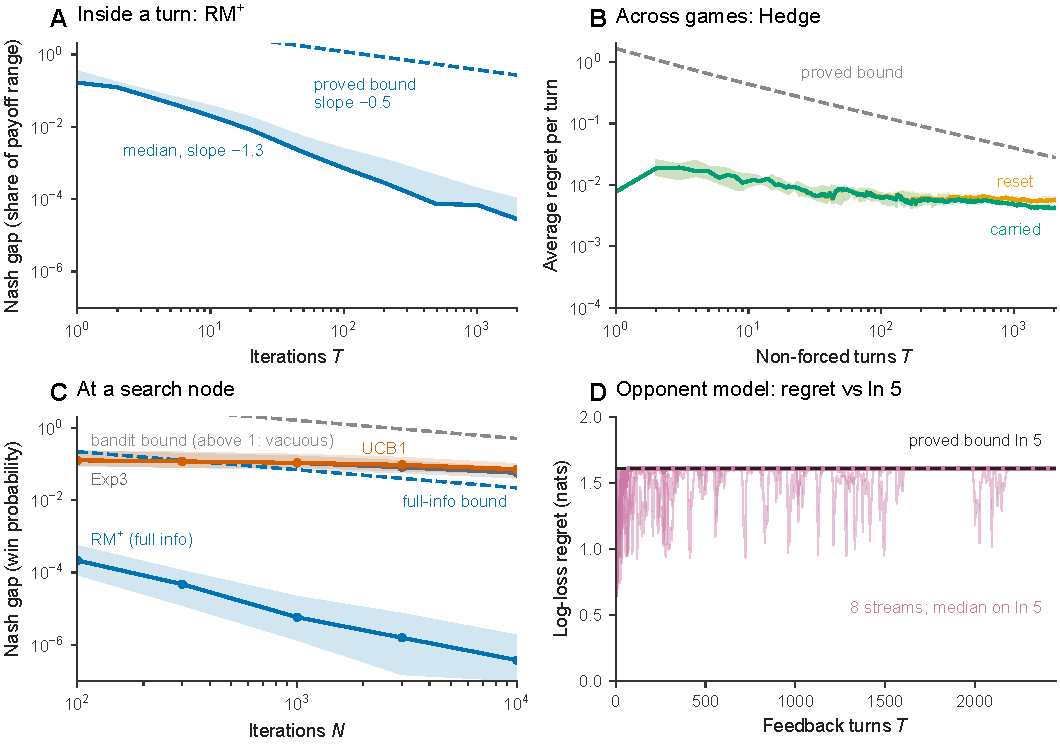
\includegraphics[width=0.9\linewidth]{fig_headline.pdf}
\caption{Regret vanishes under the proved bounds where we use no-regret learning (log--log; $y$: regret or Nash gap as
a share of the payoff range; solid: median, dashed: proved bound). \textbf{(A)} Inside a turn: Nash gap of RM$^+$'s
averaged strategy on 35 real stage matrices; band: median to 90th percentile; bound \cref{prop:rmplus}; fitted median
slope $-1.3$ against $-0.5$. \textbf{(B) Placeholder, to be replaced by E2:} average external regret per turn $R_T/T$ of
Hedge over 4 experts on surrogate rewards $\clip((q_e\cdot Ab_t-\min A)/400,0,1)$, against non-forced turns $T$; carried
versus reset weights; bound \cref{lem:R2a}, $R_T/T\le\tfrac32\sqrt{\ln k/(2T)}+\sqrt{\ln k/8}/T$ (carried learner only);
band: IQR. The plotted data are 8 replayed orders of 20 logged games (1,477 turns), not E2. \textbf{(C)} At a search node:
Nash gap of decoupled self-play on real matrices with rewards $(1+\tanh(M/160))/2$, which by \cref{prop:L4} is the
players' average regret; RM$^+$ (full information) against Exp3 and UCB1 (visit shares, one Bernoulli reward per
iteration); 100 matrices; band: IQR. Full-information reference: tuned Hedge $\sqrt{\ln n/(2N)}+\sqrt{\ln m/(2N)}$.
``Bandit bound'': the Exp3-IX high-probability bound ($\vartheta=0.05$), a reference for Exp3 and UCB1, not a bound
proved for them.}\label{fig:headline}
\end{figure}

\subsection{Structural results}\label{sec:struct}

\begin{theorem}[Theorem C and Corollary C.1: hidden information; M3; proved]\label{thm:C}
Under \cref{asm:A1}(i), \cref{asm:A4,asm:A6,asm:A7}, one-sided private information and fresh samples,
$\expl(\pi)\le\sup_\sigma\E[\sum_{t<\tau}\delta_C(t,h_t)]$ with
$\delta_C=\epss+2\epsv+2\E S_t+\eta_{\rm NL}(t)+2\Delta\TV(p_h,b^{\rm hard}_h)$. Under \cref{asm:A2,asm:A3}, the RM$^+$ and
$K$-sample rates and $\Delta=2$: $\expl(\pi)\le\Hbar\big(8\sqrt{n/T}+2\epsv+4\sqrt{2n\log K/K}\big)$. The TV term is
necessary against revealing opponents: a three-type example has $\expl=1$ while $\sum_t\eta_{\rm NL}=3/7$.
\end{theorem}
This is proof goal (i) at the game level; it is vacuous in level because $\epsv\approx1$ on exact endgames.
\begin{proposition}[S1: fixed prior; M3; proved with a named hypothesis]\label{prop:S1}
With finitely many types and a linearity cell of $v$ containing the TV ball of radius $\gamma\le\min_\theta b_\theta$
around $b$ in its relative interior, any maximiser for the $K$-sample empirical belief has
$\E[L_K]\le\Delta(2^{n_\Theta}-2)e^{-2K\gamma^2}$. The condition $\gamma\le\min_\theta b_\theta$ is necessary.
\end{proposition}
\begin{proposition}[S2: uniform over priors; M3; proved]\label{prop:S2}
On a two-type instance with one kink of slope jump 0.3, for every $c>0$,
$\liminf_K\sqrt K\sup_b\E[L_K]\ge0.3\,c\,\Phi(-2c)$, which is 0.0255 at $c^*=0.376$.
\end{proposition}
\begin{proposition}[SIM: simulator transfer; M4; exact resolution proved]\label{prop:SIM}
Under \cref{asm:A1}(i), \cref{asm:A5,asm:A6,asm:A10}, for every policy $\pi$,
$\expl_{\rm sd}(\pi)\le\expl_{\rm pe}(\pi)+\sum_{t<H}\varepsilon_{{\rm sim},t}\big(\spanop V^*_{{\rm pe},t+1}
+\sup_\sigma\spanop V^{\pi,\sigma}_{{\rm pe},t+1}\big)\le\expl_{\rm pe}(\pi)+2\Delta\sum_{t<H}\varepsilon_{{\rm sim},t}$.
At a coarsened resolution the bound needs an added within-cell oscillation term $\omega$ (proved with it; false
without it on 150 of 300 tests); the trajectory form with $\Hbar$ is a sketch.
\end{proposition}
\emph{Blend-loss bound} (M3): PIMC's one-stage loss relative to agent form was at most $4\dH$ ($\dH$ the Hausdorff
radius of the worlds' column sets) on all 46,890 logged decisions (numeric); a hand argument gives $2\dH$ (sketch).

\subsection{Levels and bridges}\label{sec:levels}

\begingroup\footnotesize
\begin{longtable}{@{}p{1.6cm}p{3.6cm}p{3.0cm}p{2.4cm}p{5.0cm}@{}}
\caption{Levels M0--M4 (M0 one exact matrix; M1 one estimated matrix, $+\epsv$; M2 full-information stochastic game,
$+$composition over $\Hbar$; M3 hidden information, $+$sampling, belief, $\eta_{\rm NL}$, prior; M4 Showdown,
$+\epssim$ and \cref{asm:A10,asm:A11,asm:A12}) and the bridges between them.}\label{tab:levels}\\ \toprule
Bridge & Crossing result & Assumptions & Status & Measurement \\ \midrule \endfirsthead
B01 M0$\to$M1 & \cref{lem:one} & \cref{asm:A7} & Lean & exact endgames only; mid-game $\epsv$ unmeasured \\
B12 M1$\to$M2 & \cref{thm:A} & \cref{asm:A1,asm:A6,asm:A7} & Lean + proved & probe: residual isolated (\cref{sec:bridges}) \\
B23 M2$\to$M3 & \cref{thm:C}, S1, S2 & \cref{asm:A2,asm:A3,asm:A4} & proved & belief accuracy (\cref{sec:belief}); Showdown oracle gap unmeasured \\
B34 M3$\to$M4 & \cref{prop:SIM} & \cref{asm:A5,asm:A10} & proved / $\omega$ / sketch & probe: KO gap $\approx0.012$ per move \\
\bottomrule
\end{longtable}
\endgroup

\paragraph{What did not transfer.} The UCB1 correlation results do not explain the engine root at practical budgets.
The 2\% $\varepsilon$-safe certificate does not survive M1$\to$M2 (SXW, \cref{sec:engine}). Rescaling the leaf toward the
TD-residual minimiser did not raise the win rate. Giving an RL best response the opponent's move distribution did not
beat black-box RL. \Cref{asm:A5} at exact-state resolution is vacuous. Theorem E2$'$ does not apply ($a=0$). Over all 70
results of the theory map: Lean 5; proved 36; proved with named hypothesis 4; proved with the $\omega$ term 1; sketch 3;
conjecture 2; numeric 8; cite 7; assumption 3; measured 1.

% =====================================================================================================
\section{Algorithms}\label{sec:alg}

All agents share one decision step (\cref{alg:turn}) and differ in the solve. Experts for Hedge are \emph{top} (argmax
row of the agent-form LP), \emph{sampled} (its mixture), \emph{safest} (pure maximin row) and \emph{safex} ($\varepsilon$-safe,
$\varepsilon=0.3\%$). \texttt{hedge} uses \cref{lem:R2a}'s anytime learner, \texttt{hedge\_fs} Hedge with fixed share
($\eta=0.2$, $\alpha=0.002$), and \texttt{hedge\_bayes} replaces safex's prediction by the style posterior's $\qhat$.
Bandit roots run decoupled UCB1 or Exp3 self-play for $N=2000$ iterations on $\bar A$ squashed to $[0,1]$ by
$(1+\tanh(\bar A/160))/2$ and play their visit shares (\texttt{\_mv} variants: the most-visited arm); \texttt{rmplus\_avg}
runs 1000 RM$^+$ iterations on the same matrix.

\begin{algorithm}[t]
\caption{One decision (agent form, with optional Hedge over experts)}\label{alg:turn}
\begin{algorithmic}[1]
\Require view of the battle; belief over opponent teams; $K$; experts $q_1..q_k$ and log-weights (if Hedge)
\Ensure a mixture $p$ over our menu, and a sampled action
\State draw worlds $\theta^{(1..K)}$ from the belief, weights $b_k=1/K$ \Comment{\texttt{hidden.determinize} / foul-play sampler}
\State $M_k\gets\texttt{nash.full\_matrix}(\theta^{(k)})$ for each $k$ \Comment{depth 2, heuristic leaf}
\State $x\gets\arg\max_x\sum_kb_k\min_j(M_k^\top x)_j$ \Comment{one LP; PIMC instead averages per-world solutions}
\If{Hedge} $p\gets\sum_ew_eq_e(\bar A)$ \Comment{$\bar A$: worlds' columns aligned (\texttt{Abar}, \texttt{run\_ourbot.py})}
\Else\ $p\gets x$ (sampled) or $e_{\arg\max x}$ (top) \EndIf
\State sample $a\sim p$; after the opponent's action $b$ is observed, update Hedge with $r_e=\clip((q_e\cdot\bar A[:,b]-\min\bar A)/400,0,1)$ \Comment{skipped if $b$ maps to no column}
\end{algorithmic}
\end{algorithm}
\emph{Cost.} Building a matrix costs about 61 ms in-engine; on Showdown a decision costs 0.2--0.3 CPU-s per side at
$K=4$, dominated by matrix construction, so agent form and PIMC cost the same (0.315 and 0.314 CPU-s per decision in E1).
The LP has $|A|+1$ variables and $\sum_k|B_k|$ constraints.

\begin{algorithm}[t]
\caption{Style posterior (\texttt{showdown/behavior.py})}\label{alg:style}
\begin{algorithmic}[1]
\Require styles $\mathcal S=\{$eq, br\_unif, br\_us, safe, uniform$\}$; temperature $\tau=0.1\,\mathrm{ptp}(\bar A)$; mix $0.05$; $\lambda=1$
\Ensure prediction $\qhat_t$ over the opponent's columns
\State each style maps $(\bar A,p)$ to $q_s$: eq = opponent's minimax $y$; br\_unif $\propto e^{-\mathrm{mean}_i\bar A_{ij}/\tau}$; br\_us $\propto e^{-(p\bar A)_j/\tau}$; safe $\propto e^{-\max_i\bar A_{ij}/\tau}$; uniform
\State mix every $q_s$ with $0.05$ uniform; $\qhat_t\gets\sum_sP_{t-1}(s)q_{s,t}$
\State after observing $b_t$: $P_t(s)\propto P_{t-1}(s)^\lambda q_{s,t}(b_t)$ (carried across games; skipped turns leave $P$ unchanged)
\end{algorithmic}
\end{algorithm}

% =====================================================================================================
\section{Experiments}\label{sec:exp}

Score is wins plus half draws of the first-named bot; games come in seat-swapped pairs with the same seed and 95\%
CIs are over pairs. In-engine games stop at 300 decision nodes (a draw). ``Stock'' is foul-play's MCTS client at
100 ms per move. Showdown scores are reported to four decimals as recorded.

\subsection{In-engine (poke-engine 0.0.48)}\label{sec:engine}

\begingroup\footnotesize\setlength{\tabcolsep}{3pt}
\begin{longtable}{@{}p{1.3cm}p{3.6cm}p{4.2cm}p{7.0cm}@{}}
\caption{In-engine experiments (full information unless stated).}\label{tab:engine}\\
\toprule ID & Question & Setup & Result [95\% CI] \\ \midrule \endfirsthead
\toprule ID & Question & Setup & Result [95\% CI] \\ \midrule \endhead
E1fix & Does the unpruned matrix fix equilibrium bots? & vs MCTS-2000; 67--74 vs 2.7 ms/move & top move 0.581 [0.540, 0.623]; safest 0.561 [0.518, 0.604]; sampled 0.443 [0.402, 0.483] (pruned matrix: 0.434, 0.302) \\
X1 & Is that win compute? & vs MCTS at 75 ms/move, 200 games each & top move 0.345 [0.289, 0.401]; safest 0.263 [0.210, 0.315] \\
E4 & Agent form vs PIMC & own tracker, $K=4$, 340 ms/move each, $n=400$ & 0.585 [0.540, 0.630]; oracle vs agent form 0.600 [0.513, 0.687] ($n=100$) \\
Blend & Does blend loss stay below $4\dH$? & all 46,890 decisions of E4 & 0 violations; max loss/bound 0.098; median loss 0.19\% of range; 61.0\% of decisions lose \\
LBR & Exploitation gain vs one-turn exploiter & 60 games per target & top 0.183 [0.10, 0.27]; sampled 0.025 [$-$0.07, 0.12]; MCTS-2000 0.160 [0.06, 0.26]; foul-play 75 ms 0.117 [$-$0.01, 0.24] \\
W1 & Certified exploitability & depth-2 white-box exploiter, 100 pairs per cell & exploiter vs top 0.873 [0.836, 0.909], vs sampled 0.713 [0.654, 0.771]; 95\% LCBs 0.250 / 0.090 (score) \\
SX & Safe exploitation vs MCTS & safex 2\%, 100 paired seeds & safex 0.530 [0.466, 0.594]; top 0.580 [0.518, 0.642]; sampled 0.510 [0.449, 0.571]; paired differences n.s. \\
SXW & Certificate vs white box & exploiter vs safex 2\%, 100 pairs & 0.767 [0.718, 0.817]; exploitability $\ge0.145$ (score) \\
LF & Leaf rescaling & vs foul-play 75 ms, 100 paired seeds & current 0.355 [0.301, 0.409]; $\tanh(h/400)$ + exact terminals 0.315 [0.259, 0.371]; difference $-0.040$ [$-0.098$, +0.018] \\
X6 & Live Hedge with per-turn feedback & 3 seeds $\times$ 80 battles, MCTS then exploiter & 0.600$\pm$0.084 vs MCTS; sampled weight overtakes top 0--3 battles after the switch \\
hedge\_ stream & Carried vs reset weights & 4 seeds $\times$ (30 vs MCTS + 30 vs exploiter) & carried $-$ reset +0.062 [$-$0.050, +0.175] vs MCTS; +0.146 [+0.039, +0.253] vs exploiter \\
rlbr\_ scale & Can RL measure exploitability? & PPO best response vs foul-play-2000, 8.01M decisions & win rate 0.060 $\to$ 0.125 [0.097, 0.153] \\
gray-box & Does seeing the opponent's distribution help RL? & as rlbr\_scale, $q$ in the input & 0.055 $\to$ 0.075 [0.051, 0.099] at 8.01M \\
\bottomrule
\end{longtable}
\endgroup

\emph{Full information.} The equilibrium top move beats MCTS-2000 only with about 25$\times$ more time per move; at
matched time MCTS wins (X1), and a value net trained on outcomes does not help (0.235 against time-matched MCTS).
Randomising costs value against a fixed opponent (sampled 0.443 vs top 0.581). By \cref{thm:A}, with RM$^+$ making
$\epss\approx0$ (\cref{fig:rmplus}), what remains is the leaf term $2\epsv\Hbar$; LF shows that error is not one of scale.

\emph{Exploitability.} This is Lecture 6's adversary in game form. Deterministic play is exploited (LBR gain 0.183,
white-box score 0.873), sampled play much less (0.025, 0.713), as \cref{thm:L6det} predicts (\cref{fig:exploit}). Sampled
play remains exploitable at $\ge0.090$ (certified), which \cref{thm:A} attributes to $\epsv$ because its stage gaps are
$\approx0$ (B12, \cref{sec:bridges}). The 2\% $\varepsilon$-safe certificate bounds loss only in $\Qhat$, and the
exploiter wins through the leaf (SXW 0.767, worse than sampled). RL best responses stay far below 0.5 and give no
useful bound.

\emph{Hidden information.} Agent form beats PIMC at equal compute (0.585), the strategy-fusion term that \cref{thm:C}
charges to PIMC; the blend-loss bound holds on every decision but is loose by $\ge10\times$. The formulation itself is
PokaiTrainer's; the head-to-head is ours.

\emph{Learners.} Carrying Hedge weights makes the learner harder to exploit (+0.146), as \cref{prop:R3d} explains;
weights move off the MCTS expert slowly against MCTS and faster once the exploiter starts (\cref{fig:hedge}).

\begin{figure}[!tbp]
\centering
\begin{minipage}[b]{0.47\linewidth}\centering
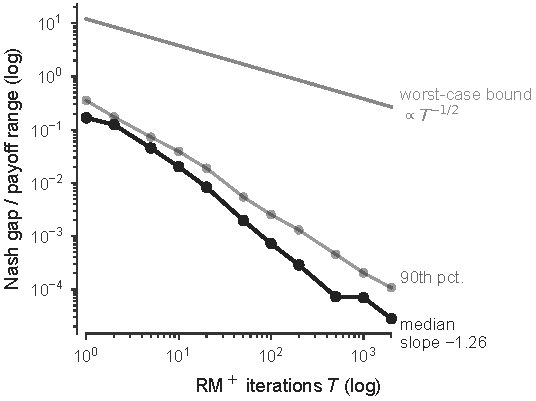
\includegraphics[width=\linewidth]{fig_rmplus.pdf}
\caption{RM$^+$ converges far faster than its worst-case bound on real stage matrices. Nash gap of the averaged RM$^+$
strategy as a share of the payoff range: median (black) and 90th percentile (gray) over 35 depth-2 matrices from
mid-game positions. Gray line: median of the proved bound $2(\sqrt n+\sqrt m)/\sqrt T$ (\cref{prop:rmplus}). Slope fitted
for $T\ge10$.}\label{fig:rmplus}
\end{minipage}\hfill
\begin{minipage}[b]{0.49\linewidth}\centering
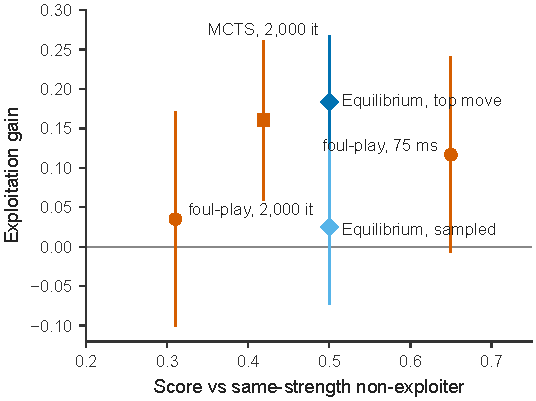
\includegraphics[width=\linewidth]{fig_exploit.pdf}
\caption{Only the deterministic bots show a significant exploitation gain. $x$: score against a same-strength
non-exploiter (0.5 by symmetry for the equilibrium bots); $y$: exploitation gain, that score minus the score against
the bot's one-turn LBR exploiter. Bars: 95\% CIs over seat-swapped pairs. Gains come from different
experiments.}\label{fig:exploit}
\end{minipage}
\end{figure}

\begin{figure}[!tbp]
\centering
\begin{minipage}[b]{0.50\linewidth}\centering
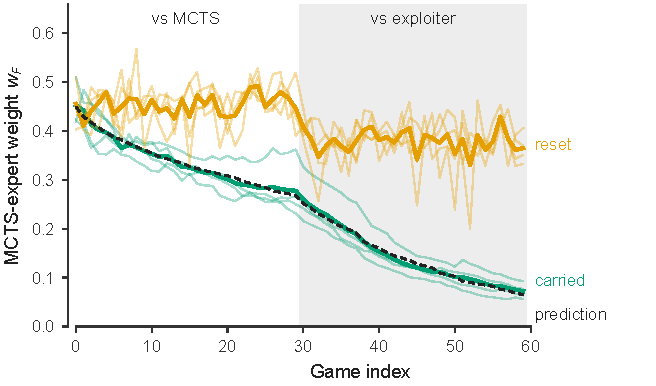
\includegraphics[width=\linewidth]{fig_hedge.pdf}
\caption{Carried weights move off the MCTS expert, faster once the exploiter starts; reset weights stay near
0.35--0.5. End-of-game MCTS-expert weight $w_F$ of Hedge over \{foul-play MCTS, equilibrium sampled\}, carried
(green) or reset each game (orange); thin lines: 4 seeds, thick: mean; shaded: games against the white-box exploiter.
Dashed: constant-drift model $w_F=\lgs(-d\sqrt{8\ln2}\sqrt t)$ with per-phase drifts fitted in-sample.}\label{fig:hedge}
\end{minipage}\hfill
\begin{minipage}[b]{0.47\linewidth}\centering
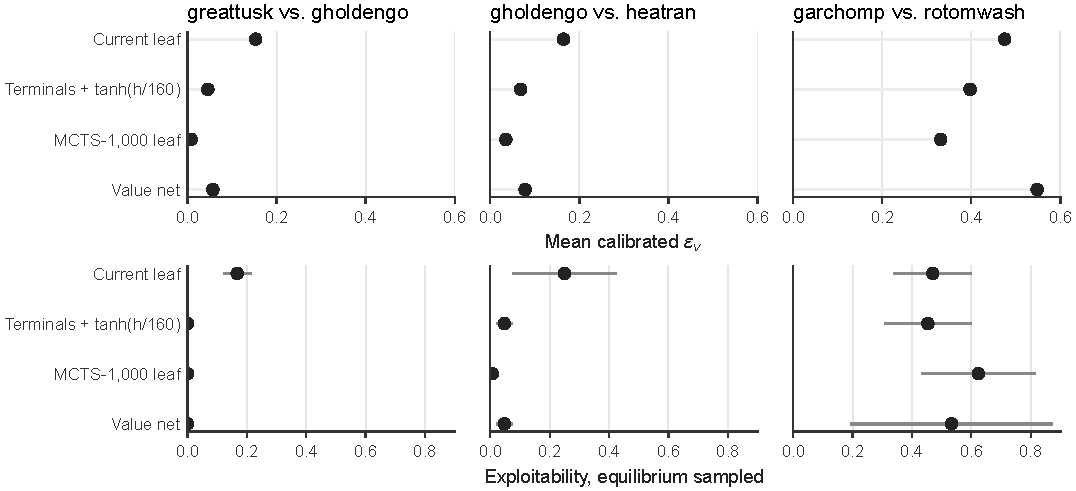
\includegraphics[width=\linewidth]{fig_leaves.pdf}
\caption{Candidate leaves on three abstracted exact endgames. Top: mean calibrated $\epsv$ (best per-state affine fit
to $Q^*$ on $[-1,1]$) over live states ($n=1{,}162$, $2{,}697$, $9{,}746$). Bottom: exploitability of equilibrium sampled
(payoff units); dot = mean of two seats, line = seat 1 to seat 2. Exact for the abstracted game, so no error bars. On
garchomp vs rotomwash no leaf lowers exploitability appreciably.}\label{fig:leaves}
\end{minipage}
\end{figure}

\subsection{Real Showdown}\label{sec:showdown}

Showdown's own simulator (commit 7e74376) runs headless; both seats use foul-play's battle tracker and set sampler
($K=4$ worlds) and our matrix per world; runs are on Modal except E1 (local).

\begingroup\footnotesize\setlength{\tabcolsep}{3pt}
\begin{longtable}{@{}p{1.25cm}p{3.6cm}p{3.7cm}p{7.5cm}@{}}
\caption{Real-Showdown experiments.}\label{tab:showdown}\\
\toprule ID & Question & Setup & Result [95\% CI] \\ \midrule \endfirsthead
\toprule ID & Question & Setup & Result [95\% CI] \\ \midrule \endhead
E1 & Agent form vs PIMC & seeds 1--300 & 0.5587 [0.5209, 0.5966], 298 pairs \\
AF & Agent form vs stock & seeds 1--300 & 0.3144 [0.2792, 0.3495], 299 pairs \\
E2 & Hedge (anytime) vs stock & 4 experts, seeds 1--400, 10 streams & 0.3108 [0.2804, 0.3412], 399 pairs; 16.43\% of feedback turns skipped \\
E2fs & Fixed-share Hedge vs stock & as E2 & 0.3033 [0.2729, 0.3336], 399 pairs; 16.83\% skipped \\
E5 & Hedge vs agent form & seeds 1--300 & 0.4583 [0.4210, 0.4956], 300 pairs, 0 errors; 17.32\% skipped \\
E4e & Exp3 root vs RM$^+$ & $N=2000$, visit shares; head-to-head & 0.0625 [0.0430, 0.0820], 296 pairs; stage gap median 0.05852, mean 0.08606 (RM$^+$ 2e-5); median top probability 0.315 vs 0.783 for RM$^+$ \\
E4u & UCB1 root vs RM$^+$ & as E4e & 0.0502 [0.0312, 0.0691], 299 pairs; gap median 0.05781, mean 0.0926; median top probability 0.225 vs 0.788 \\
E4umv, E4emv & Same, most-visited rule & \texttt{bandit\_*\_mv} & \pend \\
AF16 & Agent form with $K=16$ vs stock & & \pend \\
BH & \texttt{hedge\_bayes} vs stock, paired with E2 & seeds as E2 & \pend \\
BMstock, BMaf & Style posterior, pilot & \texttt{hedge\_bayes} vs stock / agent form, 24 pairs each & 0.3542 [0.2224, 0.4859] / 0.4792 [0.3474, 0.6109]; prediction in \cref{tab:behav} \\
BELIEF & Belief scoring run & agent form vs stock, 40 paired seeds & pair score 0.275, not a performance measure (logging overhead) \\
\bottomrule
\end{longtable}
\endgroup

\emph{Transfer of the central result.} Agent form beats PIMC on Showdown with foul-play's belief in both arms (0.5587),
so the in-engine advantage (0.585) transfers to Showdown's hidden information and a different belief model; the two
arms choose different top moves on about 11\% of decisions. \emph{Strength.} Against stock foul-play the bot loses
clearly (AF 0.3144); Hedge and fixed-share Hedge are within 0.05 of it (0.3108, 0.3033), consistent with the prediction
that Hedge stays within 0.05 of its experts, though only one expert was run alone. Feedback was skipped on 16--17\% of
turns (in E2: 2155 opponent actions in no world, 1312 fainted, 524 ``cant'', 492 no action), above the $\sim10\%$ at which
the feedback should be treated as semi-bandit, so \cref{prop:L2} applies only approximately. All 10 E2 streams end with
the top-move expert weighted highest (0.447--0.566). The pathwise regret check of \cref{lem:R2a} on the E2 logs is
\pend.

\emph{Asymmetric self-play (E5).} Hedge over experts scores 0.4583 [0.4210, 0.4956] against agent form. PA4$\beta$
predicted a score in $[0.45,0.55]$ and pre-registered a score above 0.56 as the refutation (a sign of large $\epsv$).
The prediction is not refuted and the point estimate is inside the band, but the whole CI lies below 0.5: the learner
was out-played by the equilibrium bot at 95\% confidence, an outcome the design did not anticipate. The test therefore
probes the band's lower edge, not the upper edge that PA4$\beta$ bounds.

\emph{Bandit roots (E4e, E4u).} The design compared bandit roots with RM$^+$ against an exploiter; the runs compare
them head-to-head. The bandit roots play their visit shares, whose median top probability is 0.315 (Exp3) and 0.225
(UCB1) against 0.783--0.788 for RM$^+$, with a per-turn stage gap of about 0.058 (median): this is exploration-dominated
play, and it scores 0.0625 and 0.0502. The stage gaps agree in direction with \cref{cor:B3} and are
below its 0.10--0.15. Whether MCTS's own rule, the most-visited arm, removes the loss is the pending E4umv/E4emv test.

\subsection{Behavioural model: predicting the opponent}\label{sec:behav}

The style posterior was run as part of \texttt{hedge\_bayes} in two pilots of 24 pairs. Prediction is scored
prequentially on turns with feedback (1128 against stock, 1188 against agent form; the opponent has on average 16.88
and 14.84 columns over worlds).
\begin{table}[!htbp]\centering\small
\caption{Prequential prediction of the opponent's move: log loss (nats) and argmax accuracy.}\label{tab:behav}
\begin{tabular}{@{}lcccc@{}}\toprule
 & \multicolumn{2}{c}{vs stock} & \multicolumn{2}{c}{vs agent form} \\
Predictor & log loss & accuracy & log loss & accuracy \\ \midrule
posterior $\qhat$ & 1.810 & 0.440 & 1.560 & 0.511 \\
style \emph{safe} alone & 1.810 & 0.454 & 1.558 & 0.512 \\
style \emph{br\_unif} alone & 1.816 & 0.423 & 1.697 & 0.428 \\
style \emph{eq} alone & 2.638 & 0.424 & 2.133 & 0.514 \\
uniform & 2.715 & 0.273 & 2.525 & 0.263 \\
previous predictor (one-hot br\_unif, smoothed) & 3.323 & 0.423 & 3.232 & 0.428 \\ \bottomrule
\end{tabular}\end{table}
The posterior's log loss is within 0.002 of the best single style, as \cref{prop:style} guarantees up to
$\ln5/T$ per turn, and roughly halves the previous predictor's. Against agent form, which plays a minimax mixture, the
posterior still concentrates on \emph{safe} rather than the sharper \emph{eq}: \emph{eq}'s argmax accuracy is as good
(0.514) but its probabilities are overconfident (log loss 2.133). This is consistent with the behaviour of a misspecified Bayesian posterior: it concentrates on the style with the
lowest realised log loss, here the better-calibrated one, not the ``true'' label (our interpretation). Against stock, the
two streams end on different styles (\emph{br\_unif} 0.939; \emph{safe} 0.9999), each switching at least once, which
matches the near-tie of their log losses (1.816, 1.810). Win rates of the
pilots are uninformative at 24 pairs; the full paired test is BH (\pend).

\subsection{Belief accuracy}\label{sec:belief}

\begin{table}[!htbp]\centering\small\setlength{\tabcolsep}{3.5pt}
\caption{Hidden-set beliefs scored against the truth. Not paired: simulator, generator and opponent differ between
rows. Accuracy = argmax equals truth (moves: true move among the most probable unrevealed ones).}\label{tab:belief}
\begin{tabular}{@{}llrcccc@{}}\toprule
Attribute & Belief & events & accuracy [95\% CI] & log loss & ECE & $P(\text{truth})=0$ \\ \midrule
item & foul-play posterior & 4630 & 0.838 [0.780, 0.891] & 0.257 & 0.038 & 0.002 \\
 & foul-play $K=4$ worlds & 4630 & 0.823 [0.774, 0.869] & 0.614 & 0.125 & 0.062 \\
 & ours (engine) & 9920 & 0.740 [0.680, 0.794] & 0.427 & 0.044 & 0 \\
ability & foul-play posterior & 6602 & 0.974 [0.956, 0.990] & 0.045 & 0.016 & 0 \\
 & foul-play $K=4$ worlds & 6602 & 0.971 [0.953, 0.986] & 0.077 & 0.020 & 0.006 \\
 & ours (engine) & 9920 & 0.948 [0.922, 0.970] & 0.062 & 0.007 & 0 \\
tera & foul-play posterior & 7173 & 0.633 [0.578, 0.686] & 0.627 & 0.025 & 0.001 \\
 & foul-play $K=4$ worlds & 7173 & 0.620 [0.586, 0.652] & 1.127 & 0.158 & 0.096 \\
 & ours (engine) & 9407 & 0.590 [0.503, 0.662] & 0.677 & 0.029 & 0 \\
moves & foul-play posterior & 19083 & 0.847 [0.821, 0.870] & 0.273 & 0.013 & 0.001 \\
 & foul-play $K=4$ worlds & 19083 & 0.820 [0.803, 0.839] & 0.447 & 0.089 & 0.031 \\
 & ours (engine) & 24786 & 0.683 [0.630, 0.727] & 0.480 & 0.031 & 0 \\ \bottomrule
\end{tabular}\end{table}

foul-play's posterior is accurate and calibrated (ECE 0.01--0.04, \cref{fig:belief}). The $K=4$ worlds that our Showdown
agent actually solves are not: ECE 0.09--0.16, the true value is in no world 3--10\% of the time, and log loss is
1.6--2.4$\times$ higher, although mean $P(\text{truth})$ is unchanged. The samples are unbiased, but probabilities in steps
of $1/4$ are overconfident. This is the sampling term $2\E S_t$ of \cref{thm:C}; its calibration analysis is \inprog{}
in the experts-extensions note, and AF16 ($K=16$) is the pending test. Our own tracker is calibrated within noise
in-engine (ECE 0.007--0.055); its lower accuracy reflects the engine generator's spread. Unrevealed-species belief is
near-uninformative for both (1.00--1.27 times uniform); the prior mismatch of \cref{asm:A4} is negligible (species TV at
most 0.0061).

\begin{figure}[!tbp]
\centering
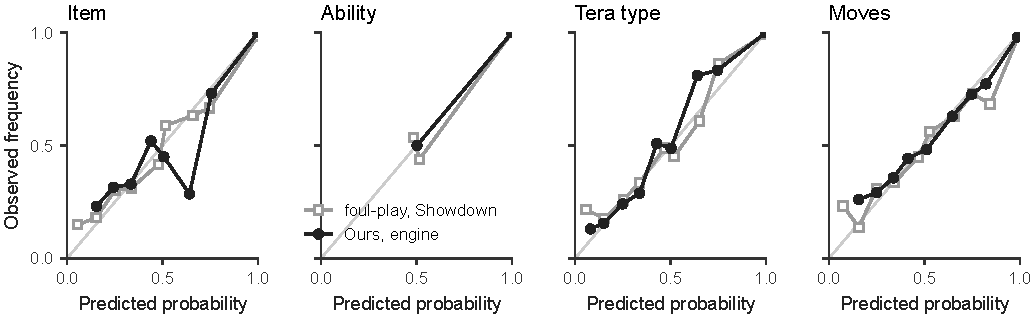
\includegraphics[width=0.78\linewidth]{fig_belief_calibration.pdf}
\caption{Hidden-set beliefs are calibrated. Observed frequency of the truth against predicted probability (10 bins)
per attribute; diagonal: perfect calibration. Gray squares: foul-play's posterior on real Showdown; black: our tracker
in-engine.}\label{fig:belief}
\end{figure}

\subsection{Bridge measurements (probe level)}\label{sec:bridges}

\emph{B12 (M1$\to$M2).} Replaying 12 logged white-box-exploiter games per target and splitting each game's loss exactly
into realised stage gain, sampling and drift terms: for sampled play the summed stage gap is 0.001 per game (median),
so all of its exploitability (0.426 in payoff units on the full log) goes through drift, the $2\epsv\Hbar$ residual of
\cref{thm:A}; for the top move the summed gap is 1.95 and the stage channel explains 0.68--1.04 of its exploitability
(0.746); for safex 2\% the per-turn gap is capped at 0.020 and exploitation goes through drift (0.534). This isolates
the residual; it does not confirm Theorem A's constant ($n=12$, noisy channel split).

\emph{B34 (M3$\to$M4).} On 21 foul-play self-play games on a local Showdown server (519 damage events, true teams
known), observed damage lies inside poke-engine's roll range in 96.5\% of events at $\pm0$ HP and 99.0\% at $\pm2$ HP;
the predicted-mean error is 2.05 HP\%; the PIT is uniform (KS $D=0.040$, $p=0.37$). The KO-indicator gap is 0.0122 per move
on average (0.011--0.015 per turn); its supremum, which \cref{asm:A5} needs, is unmeasured (observed maximum 0.31). At
exact-state resolution the mismatch is $\ge0.89$ per damaging move, so \cref{prop:SIM} is vacuous there; at KO
resolution the per-turn mean times $\Hbar\approx35$ is already 0.4--0.5.



% =====================================================================================================
\section{Discussion}\label{sec:disc}

The lectures' guarantees hold where their assumptions hold: at a single stage matrix RM$^+$ converges well inside its
bound (\cref{fig:headline}A), and across games the Hedge learner's surrogate regret falls under \cref{lem:R2a} on replayed logs (panel B, a
placeholder until E2's own curves are extracted). What
limits play is not the solver but the matrix: \cref{thm:A} and \cref{thm:C} charge every remaining loss to $\epsv$, the
exact endgames measure $\epsv$ near 1, and the B12 replay shows that a mixed bot is exploited exactly through that
channel. Lecture 6's prescription (randomise against an adaptive adversary) is confirmed in game form: sampled play has
a small exploitation gain where the top move has a large one, while against fixed opponents the top move wins.
Lecture 7's prescription works per stage but not as a search rule: a bandit root whose shares still carry exploration
scores 0.05--0.06 against full-information RM$^+$ on the same matrix, and the exploration share, not the correlation
predicted by the UCB1 analysis, explains its gap at practical budgets. The hidden-information formulation is the one
place where a structural choice paid off on real Showdown: agent form beats PIMC at equal cost, by the
strategy-fusion margin that \cref{thm:C} assigns to PIMC. The Bayesian style model adds a calibrated opponent
prediction at negligible cost, and it behaves as misspecified Bayes theory says: it chooses the best-calibrated style.

% =====================================================================================================
\section{Limitations and open problems}\label{sec:limits}

\begin{enumerate}
\item \textbf{Vacuous levels.} Every absolute bound is vacuous because $\epsv\approx1$; the theory explains rankings
and channels, not win rates. Mid-game $\epsv$ is unmeasured (poke-engine's MCTS values are root-relative).
\item \textbf{Strength.} The bot loses to stock foul-play (0.3144); matrix solving at depth 2 is not competitive with
MCTS per unit of compute.
\item \textbf{Pending:} E4umv/E4emv (most-visited rule), AF16 ($K=16$), BH (\texttt{hedge\_bayes} vs stock, paired with
E2), the E2 pathwise regret check, panel B of \cref{fig:headline}, and the experts-extensions statements marked
\inprog. Not launched: the switch test E3 and the safe-exploitation sweep PA2.
\item \textbf{$K=4$ calibration.} The worlds we solve are overconfident although the posterior is calibrated.
\item \textbf{Pivot information leak} (\cref{asm:A11}): every full-information result and the oracle see the
opponent's committed move at U-turn/Volt Switch nodes; its effect is unmeasured.
\item \textbf{Unmeasured transfer quantities:} the supremum of $\varepsilon_{{\rm sim},t}$; the oracle gap and belief TV
per turn on Showdown; $\Hbar$ in decision nodes on Showdown.
\item \textbf{Design deviations.} E4 ran head-to-head rather than against an exploiter; feedback was skipped on 16--17\%
of Hedge turns; seeded games do not replay identically across machines, so cross-machine pairing is approximate;
poke-engine's MCTS runs at least 1,000 iterations, so every ``MCTS-200'' was MCTS-1000.
\item \textbf{Proof goals (ii) and (iii)} are open beyond the sampling rates; with world-only leaves concealment has no
value in our model, so bluffing cannot be studied without belief-dependent leaves.
\end{enumerate}

% =====================================================================================================
\appendix
\section{Provenance}\label{app:prov}

\begin{sloppypar}Paths are relative to \src{cs535/final/}; SCR is the session scratchpad
\src{/private/tmp/claude-501/-Users-biofanat-Documents-classes-f26-cs535/2bbe670b-2f97-4d9a-bfad-e1139e0352c6/scratchpad/}.\end{sloppypar}
Tags: \tagV{} verified (Lean, \src{theory/CHECK.md}, the verifier pass on \src{theory/hedge_experts.md} of 2026-11-14,
or a verifier correction recorded in \src{theory/theory_map.md} \S10); \tagC{} checked by the author of this report
(recomputed from the raw logs while writing it); \tagP{} probe level, labelled ``not re-verified'' in theory\_map \S3.1;
\tagU{} unverified (including RESULTS numbers that theory\_map only restates).

\begingroup\footnotesize\setlength{\tabcolsep}{3pt}
\begin{longtable}{@{}p{4.6cm}p{9.6cm}p{0.6cm}@{}}
\toprule Numbers & Source & Tag \\ \midrule \endfirsthead
\toprule Numbers & Source & Tag \\ \midrule \endhead
Lecture statements (\cref{sec:lectures}) & \src{lecture6.pdf} \S2--4, \src{lecture7.pdf} \S2.2, \S3.2 & --- \\
Theory statements, constants, status counts (\cref{sec:theory}) & \src{theory/theory_map.md} \S4--\S9. \tagV{} applies to statements marked Lean/proved; sketch, conjecture, numeric and cite rows carry their own status (e.g.\ the S1 Weissman constant is recalled, R2a's comparison constant cited from memory) & \tagV \\
RM$^+$ slope, gap, ratio 0.04, 0.123 & theory\_map \S5.1; \src{theory/CHECK.md} finding 2; \src{report/figures/data/rmplus_gap.json} & \tagV \\
Lemma H 5.49 + 0.035S; R1 0.40; R3d 0.2966/d, 0.394 vs 0.380; P1 18--30$\times$; B3 numbers; U-fin numerics & theory\_map \S5.1, \S6, \S10 & \tagV \\
Last-iterate 0.0085 / 0.086; H4 92--99\% & theory\_map \S5.1, \S5.2 (numeric, probe) & \tagP \\
Proposition \ref{prop:style} & standard Bayes-mixture bound; \src{theory/experts_extensions.md} not yet written & \inprog \\
Game size, menu 13, difference classes & \src{theory/game_model.md} \S1.2--1.4, \S3.2 & \tagU \\
E1fix, X1, E4, blend loss, LBR gains, W1, SX, SXW, LF, X6, hedge\_stream, rlbr\_scale, gray-box, V1 0.235, 61 ms, exact endgames & \src{engine/RESULTS.md} (sections ``Fixing the payoff matrix'', ``Hidden information'', ``Blend loss'', ``Exploratory runs'', ``Foul-play-style agent'', ``Leaf value'', ``Safe exploitation'', ``Next experiments''); raw files \src{engine/results/experiments/*.jsonl}, \src{engine/results/hidden/*.jsonl}, \src{engine/results/psro/} & \tagU \\
E1 & \src{engine/showdown/results/E1_summary.json}; 11\% top-move disagreement from RESULTS ``E1'' & \tagU \\
AF, E2, E2fs, E5, E4e, E4u (scores, CIs, pairs, skip fractions and reasons, stage-gap stats) & \src{engine/showdown/results/\{AF,E2,E2fs,E5,E4e,E4u\}/*_summary.json} & \tagU \\
E4 median top probability 0.315 / 0.225 / 0.783 / 0.788 & recomputed from \src{engine/showdown/results/E4\{e,u\}/replays_headless/*.decisions.jsonl} (max of the logged \texttt{mix}) & \tagC \\
E2 final weights 0.447--0.566 & \src{engine/showdown/results/E2/hedge_state/*.json} & \tagU \\
BMstock, BMaf scores & SCR\src{behavior/work/replays_headless/BM\{stock,af\}_summary.json} & \tagU \\
\Cref{tab:behav} log loss, accuracy, scored turns, posterior trajectories (the misspecification reading is interpretation) & recomputed with SCR\src{behavior/aggregate.py} on the BM decision logs; style definitions \src{engine/showdown/behavior.py} & \tagC \\
\Cref{tab:belief}, belief findings, A4 TV & \src{engine/results/belief/report.md} & \tagU \\
BELIEF pair score 0.275 & \src{engine/results/belief/report.md} (``Caveats'') & \tagU \\
B12, B34 numbers & theory\_map \S3.1 (SCR\src{bridges/}) & \tagP \\
Figure captions & \src{report/report.tex} (rmplus, exploit, hedge, leaves); \src{report/figures/fig_headline_caption.txt}; \src{engine/results/belief/report.md} & \tagU \\
AF16, BH, E4umv, E4emv, E2 pathwise check, panel B & not yet produced & \pend \\
\bottomrule
\end{longtable}
\endgroup

\end{document}
